\chapter{SWOT}
SWOT analysis is one of the most commonly used marketing strategies. 
This analysis identifies both strengths and opportunities, and more important weaknesses and threats.\footnote{\url{http://www.businessnewsdaily.com/4245-swot-analysis.html}}
Its also important to use the information gathered in the SWOT analys to form project objectives and long term goals. 
The following SWOT analysis will be brief and will not go into detail. 
\vspace{\secspace}

\begin{figure}[H]
    \centering
    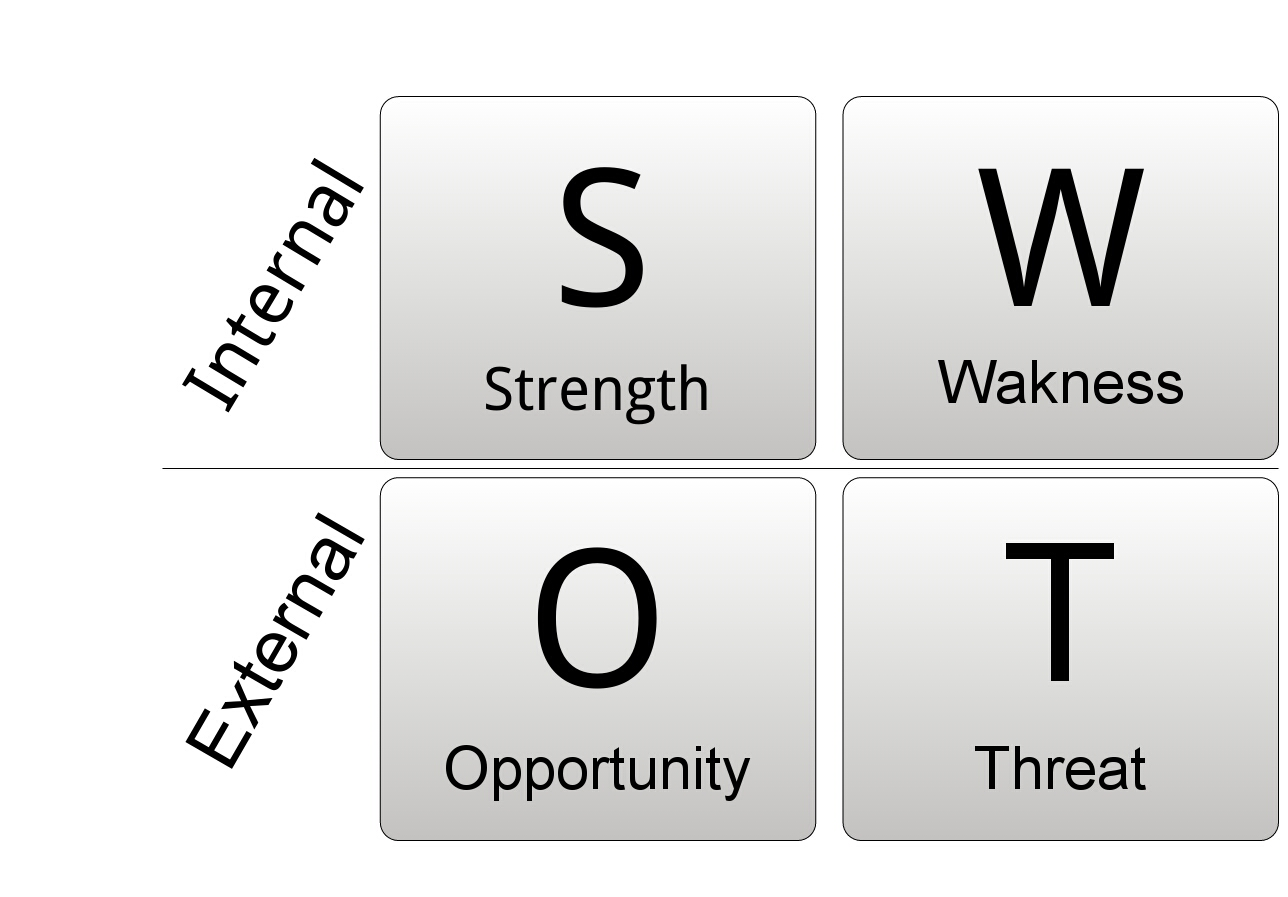
\includegraphics[width=0.6/textwidth]{graphics/SWOT.jpg}	
    \caption{SWOT}
    \label{fig:swot}
\end{figure}

\textbf{\Large Strengths}
\begin{itemize}
	 \item Everything is built on already existing technologies
	 \item Module based, which means easy to expand
	 \item Relatively cheap harware and free software
\end{itemize}

\textbf{\Large Weaknesses}
\begin{itemize}
	 \item Latency caused by http limitations
	 \item Limited to the dynamixel servos (possible to support more manufacturers)
	 \item No team to take the project further
\end{itemize}

\textbf{\Large Opportunities}
\begin{itemize}
	 \item No universal platform (that we could find) exists
	 \item Many different solutions have been tried, but no module based and easy to develope
\end{itemize}

\textbf{\Large Threats}
\begin{itemize}
	 \item Existing technologies doesnt allow easy expansion, but there are many good soluitions for different specific tasks
	 \item Marketing problems 
\end{itemize}

